%%%%%%%%%%%%%%%%%%%%%%%%%%%%%%%%%%%%%%%%%%%%%%%%%%%%%%%%%%%%%%%%%%%%%%%%%%%%%%%
% SJH-dissertation.tex - version 0.9.1.1 (5/26/2011)
%
% This is based on the template file for the osudiss-2 class. See
% osudiss-2.pdf for documentation, and the GS material 
% for the requirements.
%
% Copy the following osudiss-2 files your latex path (or just the folder containing this file):
% osudiss-2.cls (v0.9.1)
% sa-draftwater.sty
%
% Then, to compile this file:
% latex template
% bibtex template
% latex template
% latex template
%
% (You can also use pdflatex if you prefer.)
%
%%%%%%%%%%%%%%%%%%%%%%%%%%%%%%%%%%%%%%%%%%%%%%%%%%%%%%%%%%%%%%%%%%%%%%%%%%%%%%%
\documentclass[11pt, double, phd]{osudiss-2} 
% The `11pt' option is unnecessary since it is the default

% `onehalf' sets the line spacing to one-and-a-half spacing instead of
% double spacing.

% The `phd' option is unnecessary since it is the default

% Remove `draft' option for final draft

%%%%%%%%%%%%%%%%%%%%%%%%% Packages %%%%%%%%%%%%%%%%%%%%%%%%%
% Load your favorite packages here
\usepackage{graphicx} % for importing images in figures - you definitely want this!
\usepackage{lipsum} % for fake latin text---you probably don't want this
\usepackage{verbatimbox}

% For instance... see osudiss-2.pdf for some suggestions, if you don't
% have a clue
\usepackage{bm} % for bold math---useful
\usepackage{booktabs} % for more professional tables
\usepackage[titletoc]{appendix}

%hyperref packages and options
\usepackage{bookmark} % helps booksmarks look better in PDF
%hypersetup option 'breaklinks' is reguired for line wrapping in the table of contents during latex compilation, and can be removed if you use pdflatex
\hypersetup{colorlinks=true,linkcolor=blue, breaklinks} %internal links in blue, citations in green
%\hypersetup{colorlinks=true,linkcolor=black, citecolor=black, breaklinks} %all links in black
\usepackage[all]{hypcap}

%Use of natbib is STRONGLY recommended to sort and compress your references within each citation
%With these options, natbib will convert i.e. [5,3,9,4] to [3-5, 9]
\usepackage[sort&compress]{natbib}

%required to have latex automatically generate subfigures (i.e. (a), (b) etc)
\usepackage{subfig}
\usepackage[export]{adjustbox}
\setcounter{lofdepth}{2}
\PassOptionsToPackage{obeyspaces}{url}
%\usepackage{hyperref}% http://ctan.org/pkg/hyperref

%load glossaries packages
\usepackage[acronym, section=chapter]{glossaries}
%\usepackage[xindy,acronym, section=chapter]{glossaries} - recommended if supported by your OS
\makeglossaries %required to actually make a glossary
%A list of common acronyms
%Only those used will be displayed, so you can just add to this list
\newacronym{fwhm}{FWHM}{full-width-at-half-maximum}
\newacronym{fft}{FFT}{Fast Fourier Transform}
\newacronym{swpg}{SWPG}{square-wave phase grating}
\newacronym{cats}{CATS}{Complex Attoseond Transient-absorption Spectroscopy}
\newacronym{ir}{IR}{infrared}
\newacronym{doe}{DOE}{diffractive optical element}
\newacronym{hhg}{HHG}{high-harmonic generation}
\newacronym{table}{TABLe}{transition-absorption beamline}
\newacronym{vls}{VLS}{variable line spaced}
\newacronym{mcp}{MCP}{microchannel plate}









 %load list of acronyms contained in acronyms.tex

%The following commands can be used to help deal with "overfull hbox" issues
%See, for example, http://www.tex.ac.uk/cgi-bin/texfaq2html?label=overfull for details
%\pretolerance 1000
\setlength{\emergencystretch}{3em}
%\tolerance 1000

%%%%%%%%%%%%%%%%%%%%%%%%% Custom Commands/Environments %%%%%%%%%%%%%%%%%%%%%%%%%
% Put your favorite custom commands here
%\newcommand{\fish}{\alpha} % some of my students call it the "fish" symbol

%Print list of abbreviations - use same font as List of Figures and List of Tables for the title, and same formatting in the table of contents.
% Argument #1 - title for list of abbreviations (i.e. List of Abbreviations)

\newcommand\PrintListofAbbreviations[1]{
\phantomsection
\addcontentsline{toc}{front}{\typesetColumnHeading{#1}}
\printglossary[type=\acronymtype,title={\protect {\typesetLevelTwo{#1}}}]
}


\newenvironment{chapabstract}{%
    \begin{center}%
      \bfseries Abstract
    \end{center}}%

% Below is an example of customizing the style of headings in your
% dissertation. See osudiss-2.pdf for more information.
%
% For example, if you simply must have uppercase titles:
%\renewcommand\typesetLevelOne[1]{{\Large\textbf{\MakeUppercase{#1}}\par}}
%\renewcommand\typesetLevelTwo[1]{{\Large\textbf{\MakeUppercase{#1}}}}
% Note the \par for \typesetLevelOne
%
% If you want the title to be bold and |\Large| instead of |\Huge|:
%\renewcommand\titleFont{\normalfont\Large\bfseries}

% Add words that TeX may not know how to hyphenate below. This can
% help prevent overfull hboxes. For example,
\hyphenation{eigen-state space-time} 

%%%%%%%%%%%%%%%%%%%%%%%%% Document Metadata %%%%%%%%%%%%%%%%%%%%%%%%%
\title{Attosecond transient absorption spectroscopy}
\author{Stephen J. Hageman}
\advisorname{Louis F. DiMauro}
\degree{Doctor of Philosophy} % Default value
\member{Douglass Schumacher}
\member{Jay Gupta}
\member{Robert Baker}
\authordegrees{M.Sc.}
\graduationyear{2019}
\unit{Graduate Program in Physics} 

%%%%%%%%%%%%%%%%%%%%%%%%% Begin Document %%%%%%%%%%%%%%%%%%%%%%%%%
\begin{document}
\showthe\textwidth
\frontmatter

\begin{abstract}

An experimental technique is developed to measure the complex refractive index in a transient-absorption experiment using attosecond pulse trains.  This complex attosecond transient-absorption spectroscopy (CATS) method is demonstrated by measuring the dynamic change, induced by an infrared dressing pulse, in the real and imaginary parts of the refractive index of the argon $3s3p^6np$ Fano resonances.  Typical attosecond transient-absorption spectroscopy (ATS) measurements only capture the imaginary part of the refractive index, and the real part can only be indirectly calculated.  CATS enables a direct measurement of the real part of the refractive index, and this removes the need to rely upon indirect calculations which are only valid if certain assumptions hold true.  While CATS is demonstrated in a gas phase experiment, it can also be used for condensed matter experiments in either a transmission or reflection geometry.

As a prelude to the demonstration of CATS, an ATS experiment is performed to examine the dynamics of the argon $3s3p^6np$ Fano resonances under the influence of a dressing field.  This ATS measurement reveals a complicated structure of light-induced states and light-induced attenuation in the intensity and time delay dependence of the absorption spectrum.  The theoretical understanding of these features is detailed, and excellent agreement between theoretical and experimental results is demonstrated. 

Additionally, the optical tool that enables CATS to be performed is detailed theoretically and experimentally. This tool is a diffractive optical element known as a $0-\pi$ square-wave phase grating (SWPG).  The SWPG allows for an input femtosecond IR pulse to be duplicated, and the SWPG can control the relative phase between these duplicates.  This relative phase control is demonstrated, and it is used to measure the ground state complex refractive index of silicon and germanium.


\end{abstract}

\dedication{Dedicated to coffee} % Optional, and seriously not this lame
\begin{acknowledgments}

First of all, I would like to thank both my advisor and my emeritus advisor, Lou DiMauro and Pierre Agostini, for all of their support throughout my time in graduate school. I have gotten to work with a wonderful cast of characters during my time in graduate school, and I wouldn't be where I am today without them.

I'd particularly like to acknowledge the friends that I have made while in graduate school: Thuc Mai, Tim Gorman, Alex Dyhdalo, Steve Tjung, Matt Sheffield, Solani Harawa, and Greg Smith.  I truly cherish the time that we have spent together, and I couldn't have asked for a better friend group.  I truly appreciate your friendship, and I know that graduate school would have been a worse experience without you.

I would also like to thank the members of the group that have helped me along the way: Dietrich Kiesewetter, Antoine Camper, Hyunwook Park, Yu Hang Lai, Sha Li, Cosmin Blaga, Kent Talbert, Eric Moore, Kaikai Zhang, Junliang Xu, Abraham Camacho, Sierra O'Bryan, Andrew Piper, Daniel Tuthill, Tim Scarborough, Zhou Wang, Yagou Tang, and Stephen Schoun.  Each and every person in the group has provided invaluable help to me as I navigated my way through research.

I wouldn't have made it through graduate school without the help of machinists Mike Graham and Pete Gosser.  They are truly the ones who deserve credit for the TABLe.  They went above and beyond to help Greg and me when we were designing it, and it was awesome to work with them on such a large project.

It is important that I acknowledge the contributions of my parents and my sister: Jim, Beth, and Jennifer Hageman.  They have provided endless support to me, and they have helped shape the person I am today.  They have always encouraged me to follow my passions, and I will be eternally grateful for that.

I would also like to thank Wallace and Ricky Hageman.  They have been by my side throughout graduate school, and they have always been there when I needed some support. They inspired some of the acronyms used throughout this dissertation.

Finally, I would like to thank Rileigh.  Without graduate school, I wouldn't have met her, and without her, graduate school wouldn't have been the same.  Her belief in me helped carry me through some dark days, and I am eternally grateful that she is by my side.


%I would like to thank Sir Rickenabcker First of His Name, Last of His Kind, for his eternal indifference.


\end{acknowledgments}
\begin{vita}
%\dateitem{Oct 17, 1990}{Born---Kolkata, India}
\dateitem{2011}{Bachelors of Science in Physics and Mathematics, Johns Hopkins University}

\dateitem{2014}{Master of Science in Physics, The Ohio State University}
\dateitem{2014 to present}{Graduate Research Associate, The Ohio State University}
% Insert other relevant items here (GTA, etc.)

\begin{publist}

\pubitem{Vyacheslav E. Leshchenko, Bradford K. Talbert, Yu Hang Lai, Sha Li, Yagou Tang, \textbf{Stephen J. Hageman}, Greg Smith, Pierre Agostini, Louis F. DiMauro, and Cosmin I. Blaga. ``Cr:ZnSe mid-IR, multi-mJ, few-cycle amplifier: a new platform for attosecond soft-X-ray physics," Optica 7 (8), 981-988 (2020)}

\pubitem{Antoine Camper, Hyunwook Park, \textbf{Stephen J. Hageman}, Greg Smith, Thierry Auguste,
	Pierre Agostini, and Louis F. DiMauro. ``High relative-phase precision beam duplicator
	for mid-infrared femtosecond pulses." Optics Letters, 44 (22), 5465-5468 (2019)}

\pubitem{B. Peters, A. Alfonsov, C. G. F. Blum,\textbf{ S. J. Hageman}, P. M. Woodward, S. Wurmehl, B. Büchner, and F. Y. Yang, ``Epitaxial films of Heusler compound Co$_{2}$FeAl$_{0.5}$Si$_{0.5}$ with high crystalline quality grown by off-axis sputtering,” Appl. Phys. Lett. 103, 162404 (2013)}
\pubitem{W. G. Wang, A. Pearse, M. Li, \textbf{S. Hageman}, A. X. Chen, F. Q. Zhu, and C. L. Chien, ``Parallel fabrication of magnetic tunnel junction nanopillars by nanosphere lithography,” Scientific Report 3, 1948 (2013)}
\pubitem{W. G. Wang, M. Li, \textbf{S. Hageman}, and C. L. Chien, "Electric-field-assisted switching in magnetic tunnel junctions," Nature Mater. 11, 64 (2012)}
\pubitem{W. G. Wang, \textbf{S. Hageman}, M. Li, S. X. Huang, X. M. Kou, X. Fan, J. Q. Xiao, and C. L. Chien, ``Thermal annealing study of magnetoresistance and perpendicular anisotropy in magnetic tunnel junctions based on MgO and CoFeB," Appl. Phys. Lett. 99, 102502 (2011)}


\end{publist}


\begin{fieldsstudy}
\majorfield{Physics}
%\onestudy{Particle Astrophysics}{Connolly group} % optional
% Alternatively you can do:
\end{fieldsstudy}

\end{vita}

\tableofcontents 

% list of figures (comment out if you don't have any figures)
\clearpage %remove if you don't want a page break before list of figures
\listoffigures 

% list of tables (comment out if you don't have any tables)
%\clearpage  %remove if you don't want a page break before list of tables
%\listoftables 

%print glossary - comment out if you don't want this.  Make sure you also add \glsdisablehyper if you don't want to print a glossary, but do use the %glossaries package to keep track of acronyms
\clearpage %remove if you don't want a page break before list of abbreviations
\PrintListofAbbreviations{List of Abbreviations} %Title is in { } - change if desired
%\printglossary[type=\acronymtype]

\mainmatter
\chapter{Introduction}

\section{Exciting astrophysics happen far, far away}

We live in a boring part of the Universe. This allows life and the life sciences to thrive here. However, everything that is interesting in astrophysics takes place far, far away. For example, most \gls{grbs} take place about 1 Gpc \ref{anita2} away from us. That is over three billion light years away! 



\begin{figure}
\centering
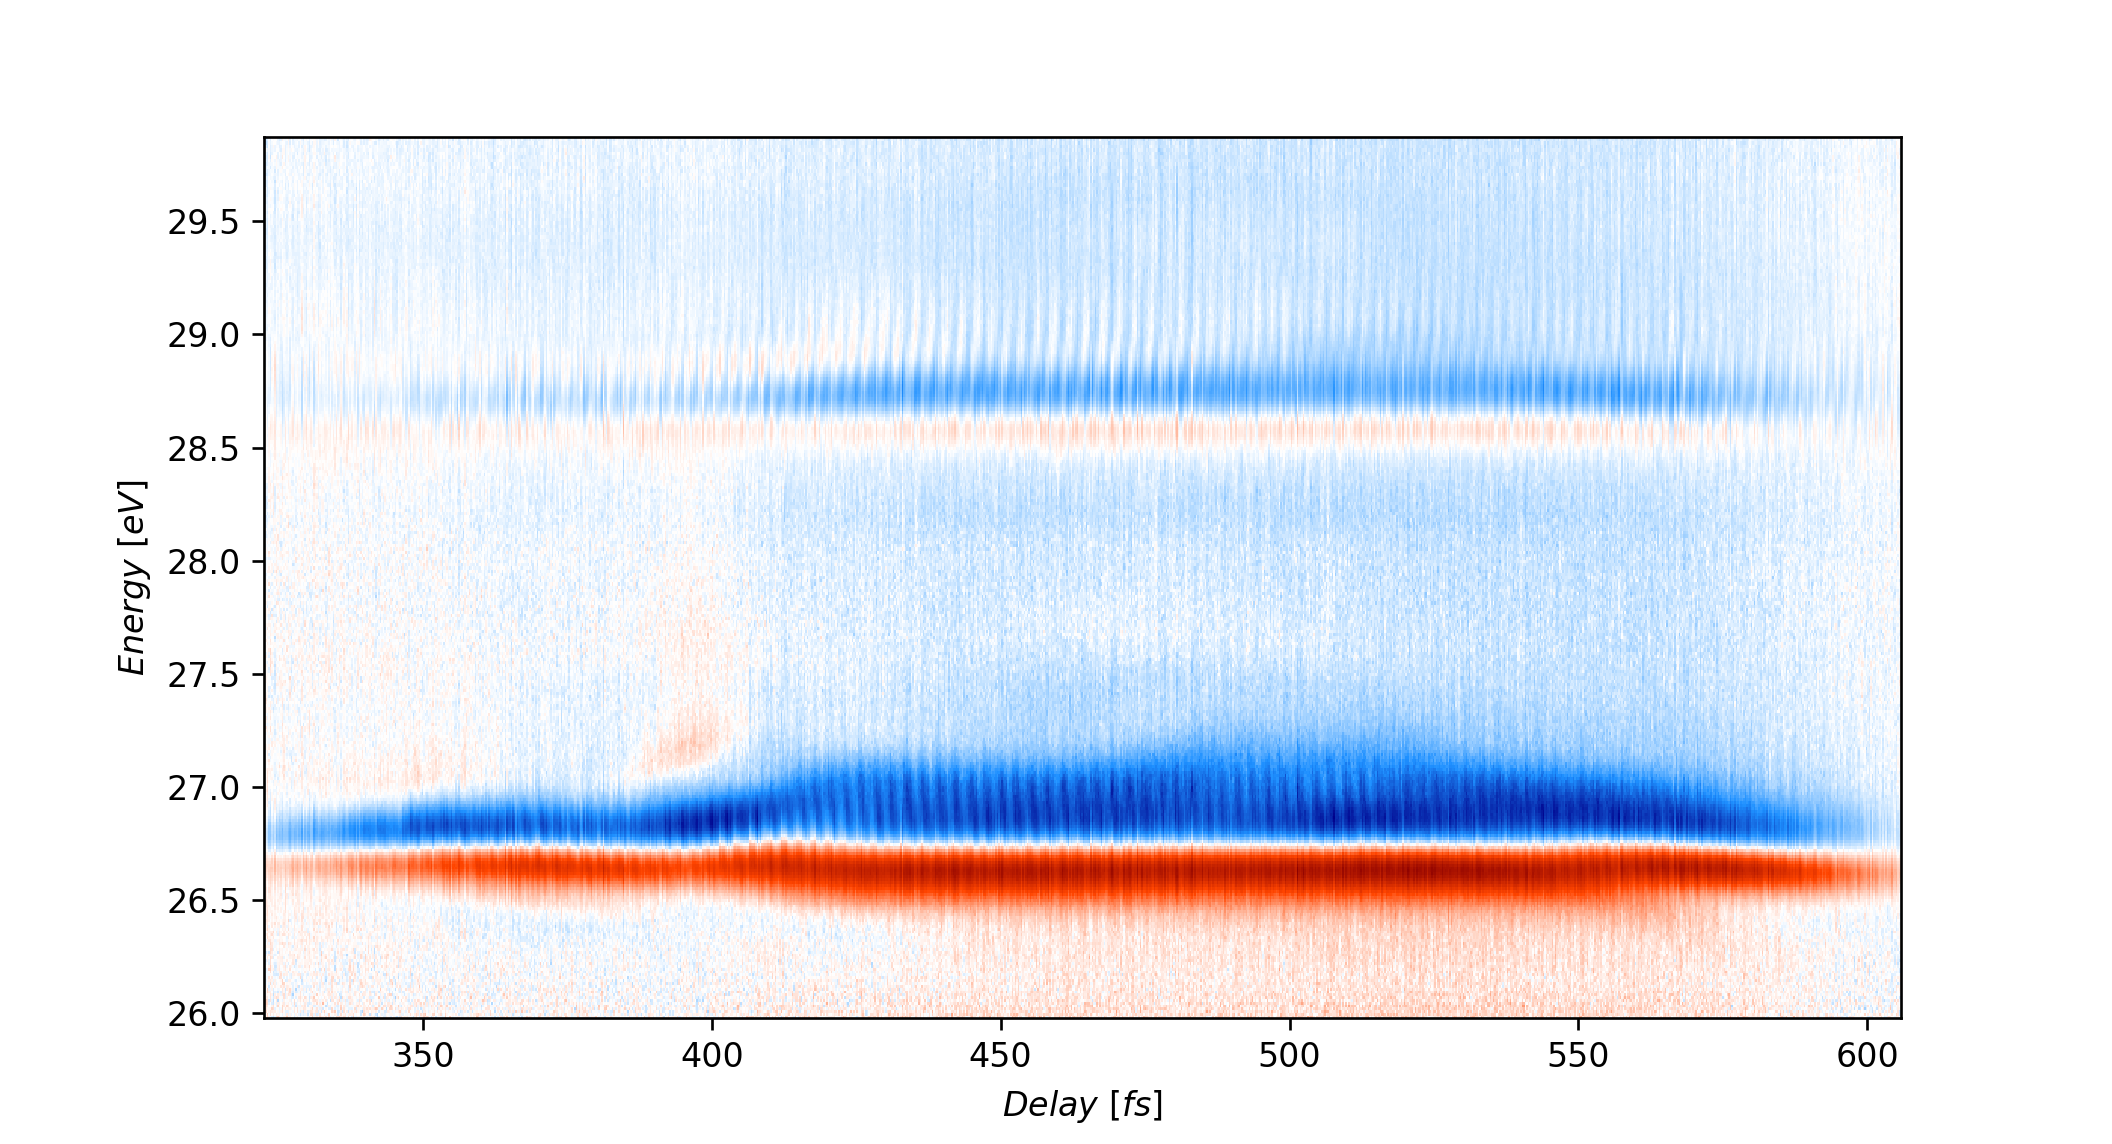
\includegraphics[width=0.5\textwidth]{figures/Introduction/6_forthesis.png}
\caption{Depiction of a GRB. Picture Credit: NASA E/PO, Sonoma State University, Aurore Simonnet.}
\label{grb}
\end{figure}

\section{Astrophysical messengers}

Traditional astrophysical messengers are not able to completely probe physics that take place at the farthest distances and at the highest energies. Since the beginning of astronomy, we have relied on optical light to study objects in the sky. In the last few decades, we have started utilizing light of other wavelengths such as X-rays and gamma rays. However, light of energy 1~MeV and above can undergo pair production. Light of energy 13.6~eV gets absorbed by Hydrogen atoms, the most abundant element in the Universe, while light at other wavelengths gets absorbed by other atoms and molecules. Light is the astronomer's best friend, but there is an inevitable need for complementary messengers.

Fortunately, in the last century, we have opened up multiple new windows t

%\begin{figure}
%\centering
%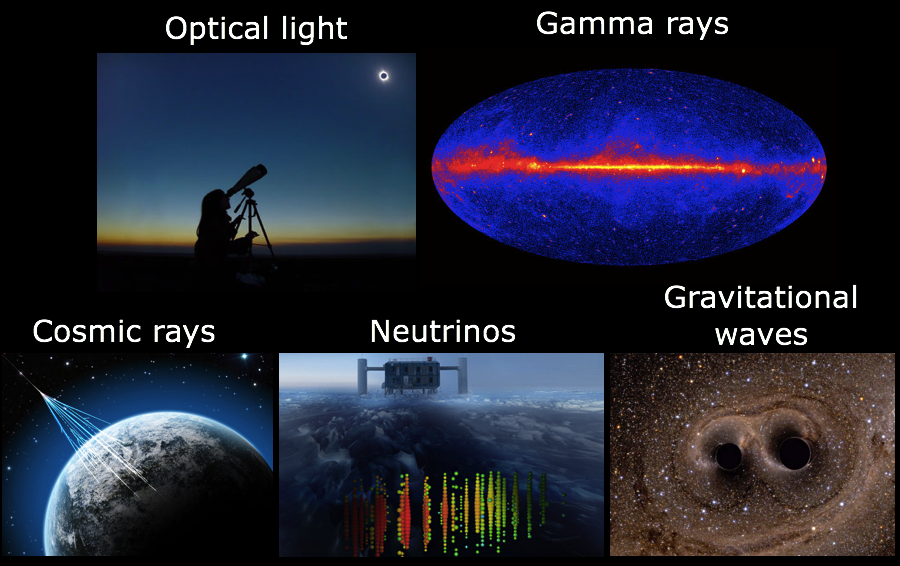
\includegraphics[width=1.0\textwidth]{figures/messengers.png}
%\caption{Astrophysical messengers. Pictures are all borrowed from Fermi, IceCube and LIGO collaborations, and the Internet.}
%\label{messengers}
%\end{figure}

\begin{figure}
\centering
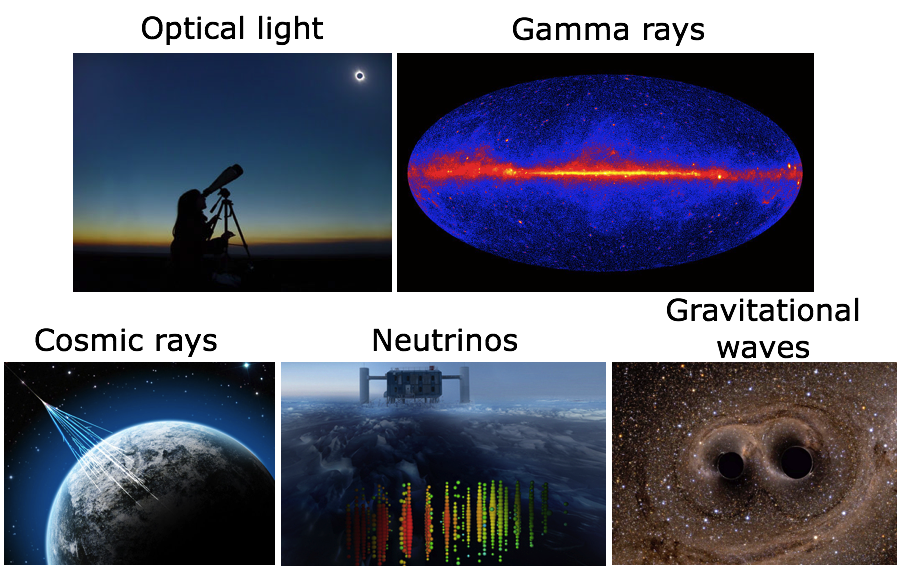
\includegraphics[width=1.0\textwidth]{figures/messengers_2.png}
\caption{Astrophysical messengers. Pictures are all borrowed from Fermi, IceCube and LIGO collaborations, and the Internet.}
\label{messengers}
\end{figure}

\section{Neutrinos as astrophysical messengers}

Neutrinos are potentially perfect candidates for carrying information about distant particle accelerators all the way to us. Due to being neutral and weakly interacting, neutrinos would remain unattenuated and point straight back to their source. In this way, they would have a definite advantage over messengers such as cosmic rays. Neutrinos are the side product of almost every nuclear reaction and can carry versatile information about particle physics taking place at cosmic distances. Their  

\begin{figure}
\centering
\subfloat[t]{
	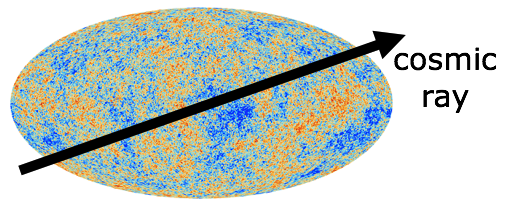
\includegraphics[width=0.8\textwidth, valign=c]	{figures/cosmogenic_2.png}
    \label{cosmogenic}
    }\quad
\subfloat[b]{
	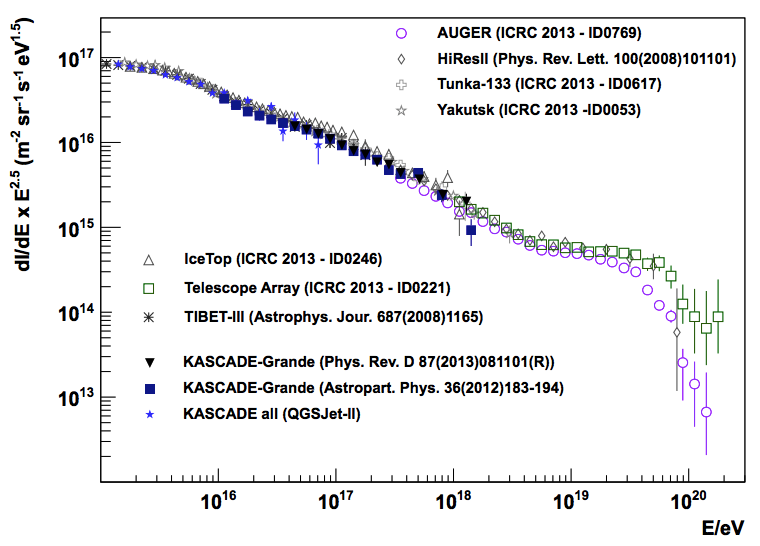
\includegraphics[width=0.8\textwidth, valign=c]{figures/kneeankle.png}
    \label{kneeankle}
    }
\caption{Top: Depiction of a cosmic ray interacting with the CMB. Thanks to the Planck telescope for the CMB picture. Bottom: Energy spectra of cosmic rays measured by different experiments. Andreas Haungs showed this plot at the 13th International Conference on Topics in Astroparticle and Underground Physics. UHE cosmic rays can only travel for about 50 Mpc before they interact with CMB photons and lose energy, therefore, we see a sharply falling spectrum at about $10^{20}\,\mbox{eV}$ energy.}
\label{cr}
\end{figure}

\begin{figure}
\centering
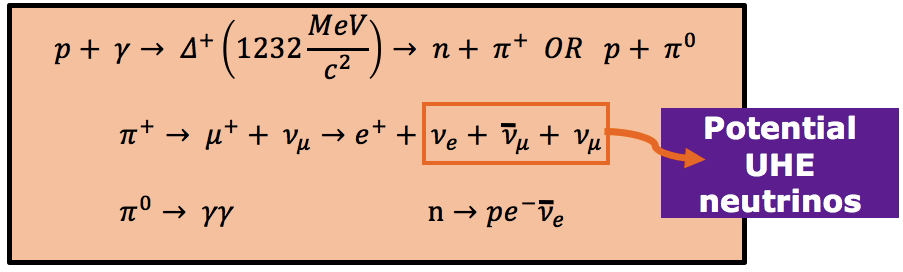
\includegraphics[width=1.0\textwidth]{figures/uhe_process.png}
\caption{A process for production of UHE neutrinos.}
\label{uhe_process}
\end{figure}

\section{Optical Cherenkov neutrino detectors}


IceCube and ANTARES are both optimized for the detection of muons from charged current interactions of high energy astrophysical neutrinos. IceCube uses the Antarctic ice as a target medium for high energy neutrinos to interact in. ANTARES uses sea-water instead. They both look for optical Cherenkov signatures of high energy neutrino interactions. ANTARES is sensitive to neutrinos of energy 10 GeV - 100 TeV. IceCube was built ceCube can also detect neutrinos of energy of order MeV. 


\begin{figure}
\centering
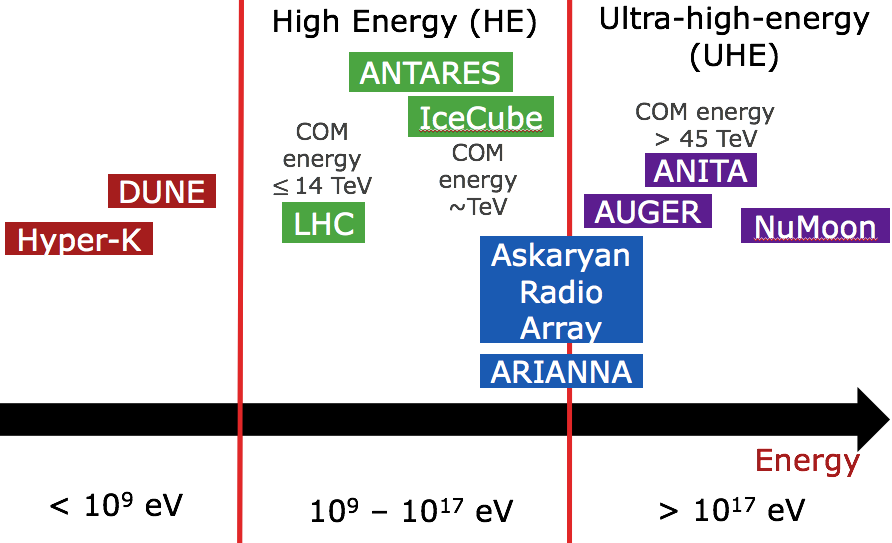
\includegraphics[width=0.9\textwidth]{figures/anita_where_energy.png}
\caption{The ANITA experiment looks for particles, specifically, neutrinos of energies that are to close to the extreme right of the energy scale.}
\label{anita_energy}
\end{figure}


\section{Radio Cherenkov neutrino detectors}

Radio Cherenkov neutrino experiments look for \gls{uhe} neutrinos in the energy regime of $> 10^{16}\,\mathrm{eV}$. The main challenge for detection by these experiments and a potential solution for detection are presented below. We also introduce two complementary radio Cherenkov experiments,andin this section. Where they are on the energy scale as compared to other particle physics experiments is shown in Figure



\subsection{Askaryan Effect}

f light in the medium. The particle shower would mainly consist of photons, electrons and positrons. As it travels through the dielectric, the particle shower develops about a 20\% negative charge. This happens primarily due to Compton scattering of electrons in the medium (so electrons leaving the medium and joining the shower) and secondarily due to annihilation of positrons in the shower with electrons in the medium (so positrons leaving the shower).   
As this charged particle shower travels through the medium at a speed greater than the speed of light in the medium, Cherenkov radiation is produced. If this Cherenkov radiation is observed at wavelengths larger than the shower's transverse dimension of about 10 cm, then it would be seen as coherent waves in radio frequencies. 

\begin{figure}
\centering
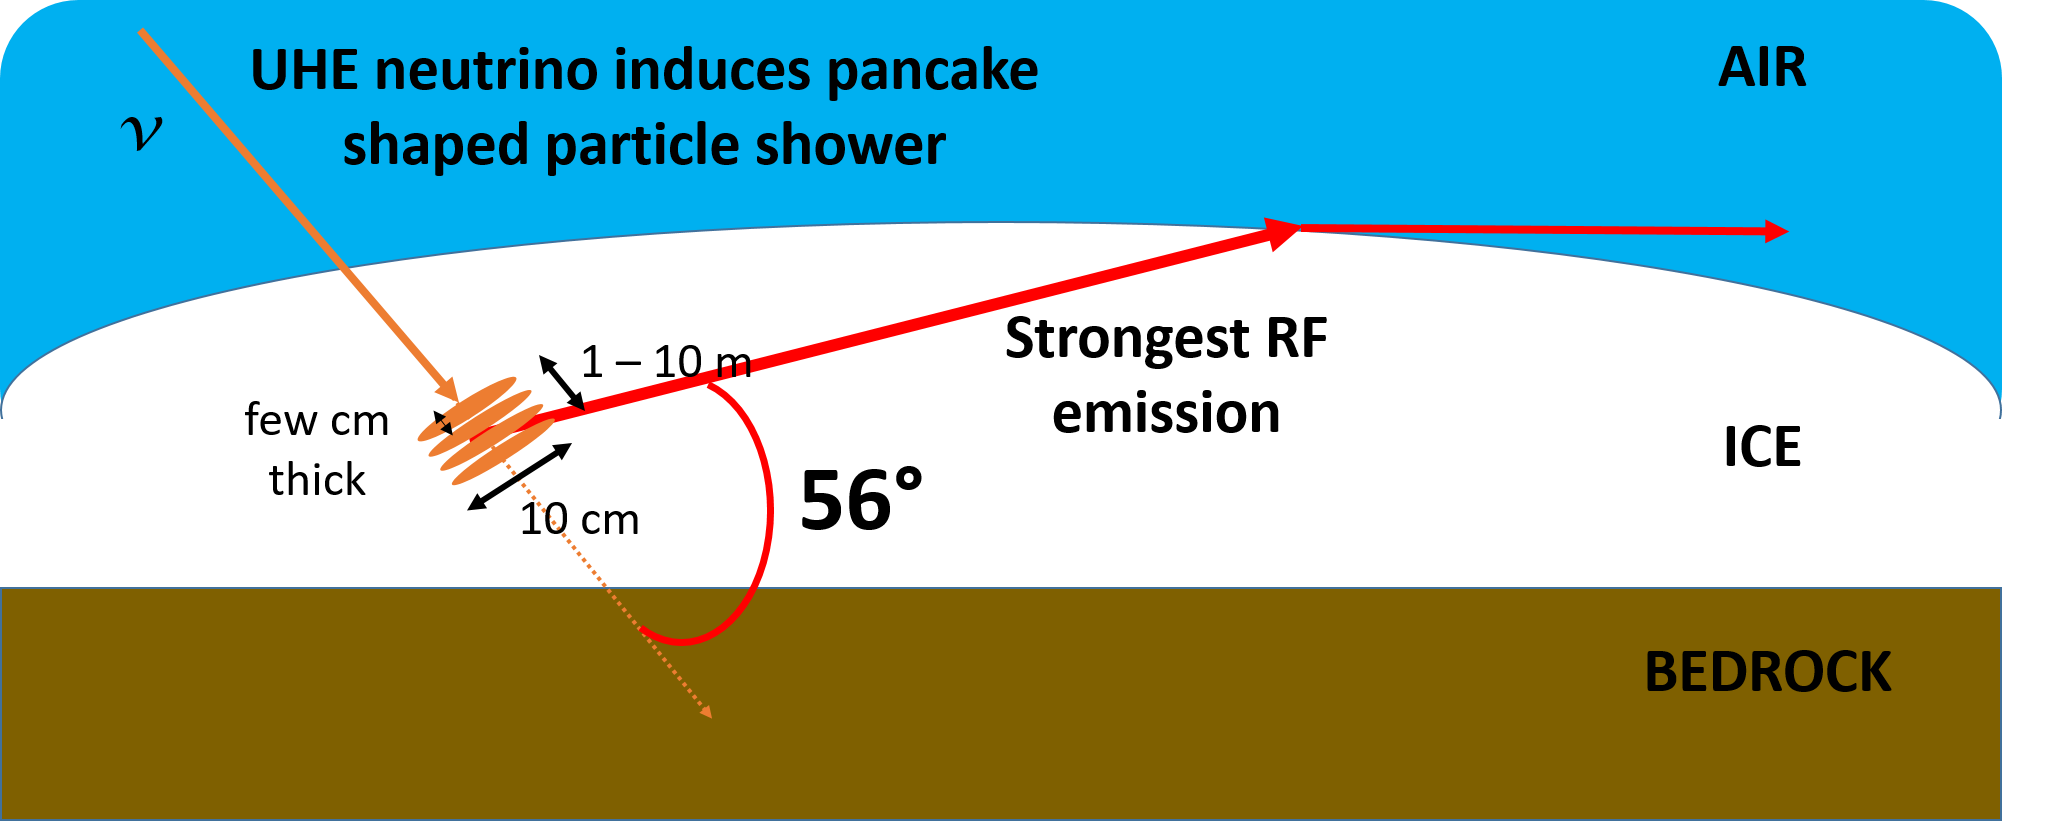
\includegraphics[width=1.0\textwidth]{figures/askaryan_in_ice.png}
\caption{A UHE neutrino could start a pancake-shaped particle shower in the ice.
Cherenkov radiation due to this particle shower would be coherent at wavelengths 
greater than the shower size of $\sim~10\,\mbox{cm}$, which correspond to radio waves.}
\label{askaryan}
\end{figure}

%ANITA and ARA use radio techniques to look for high energy neutrinos on the higher end of the energy spectrum as shown in Figure~\ref{anita_energy}. ARA covers the energy range $10^{16} - 10^{19}\, \mathrm{eV}$ which includes part of the UHE region and ANITA covers the UHE region from $10^{18}\, \mathrm{eV}$ and above. Below we provide a brief overview of these different experiments and how they complement one another.

\subsection{ANITA}

fect utilizing the Antarctic ice as the necessary dielectric target medium for neutrino interaction. Where \gls{anita}'s sensitivity lies in the energy scale as compared to other experiments in particle physics and particle astrophysics is presented in Figure=. A cartoon of an]oats up to an altitude of about 40 km and utilizes the polar vortex to fly in roughly circular orbits over the continent of Antarctica. At its float altitude, the balloon, upon gradual inflation, is bigger than the Ohio Stadium. There have been four flights of \gls{anita} so far. These are summarized in Figure

\begin{figure}
\centering
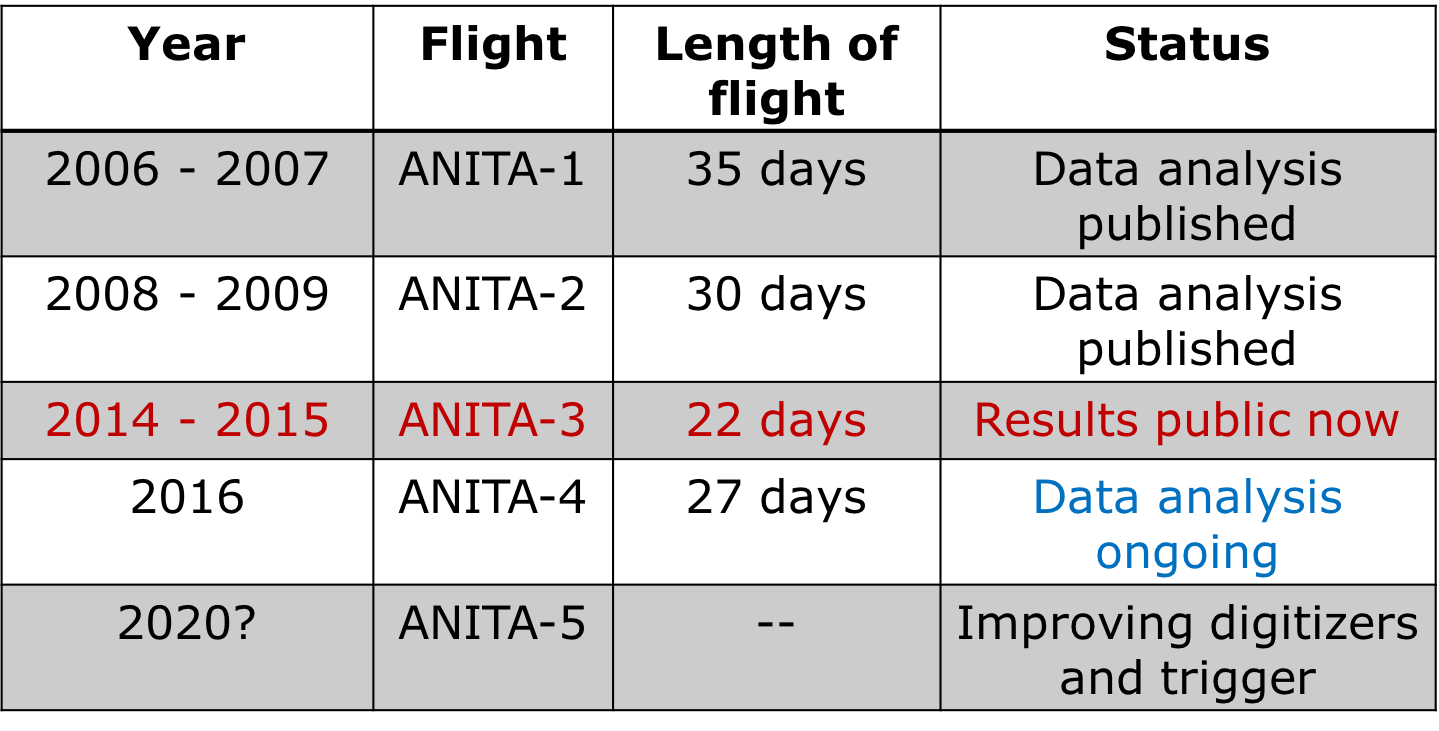
\includegraphics[width=1.0\textwidth]{figures/flights_table.png}
\caption{Summary of ANITA flights.}
\label{flights_summary}
\end{figure}


\begin{figure}
\centering
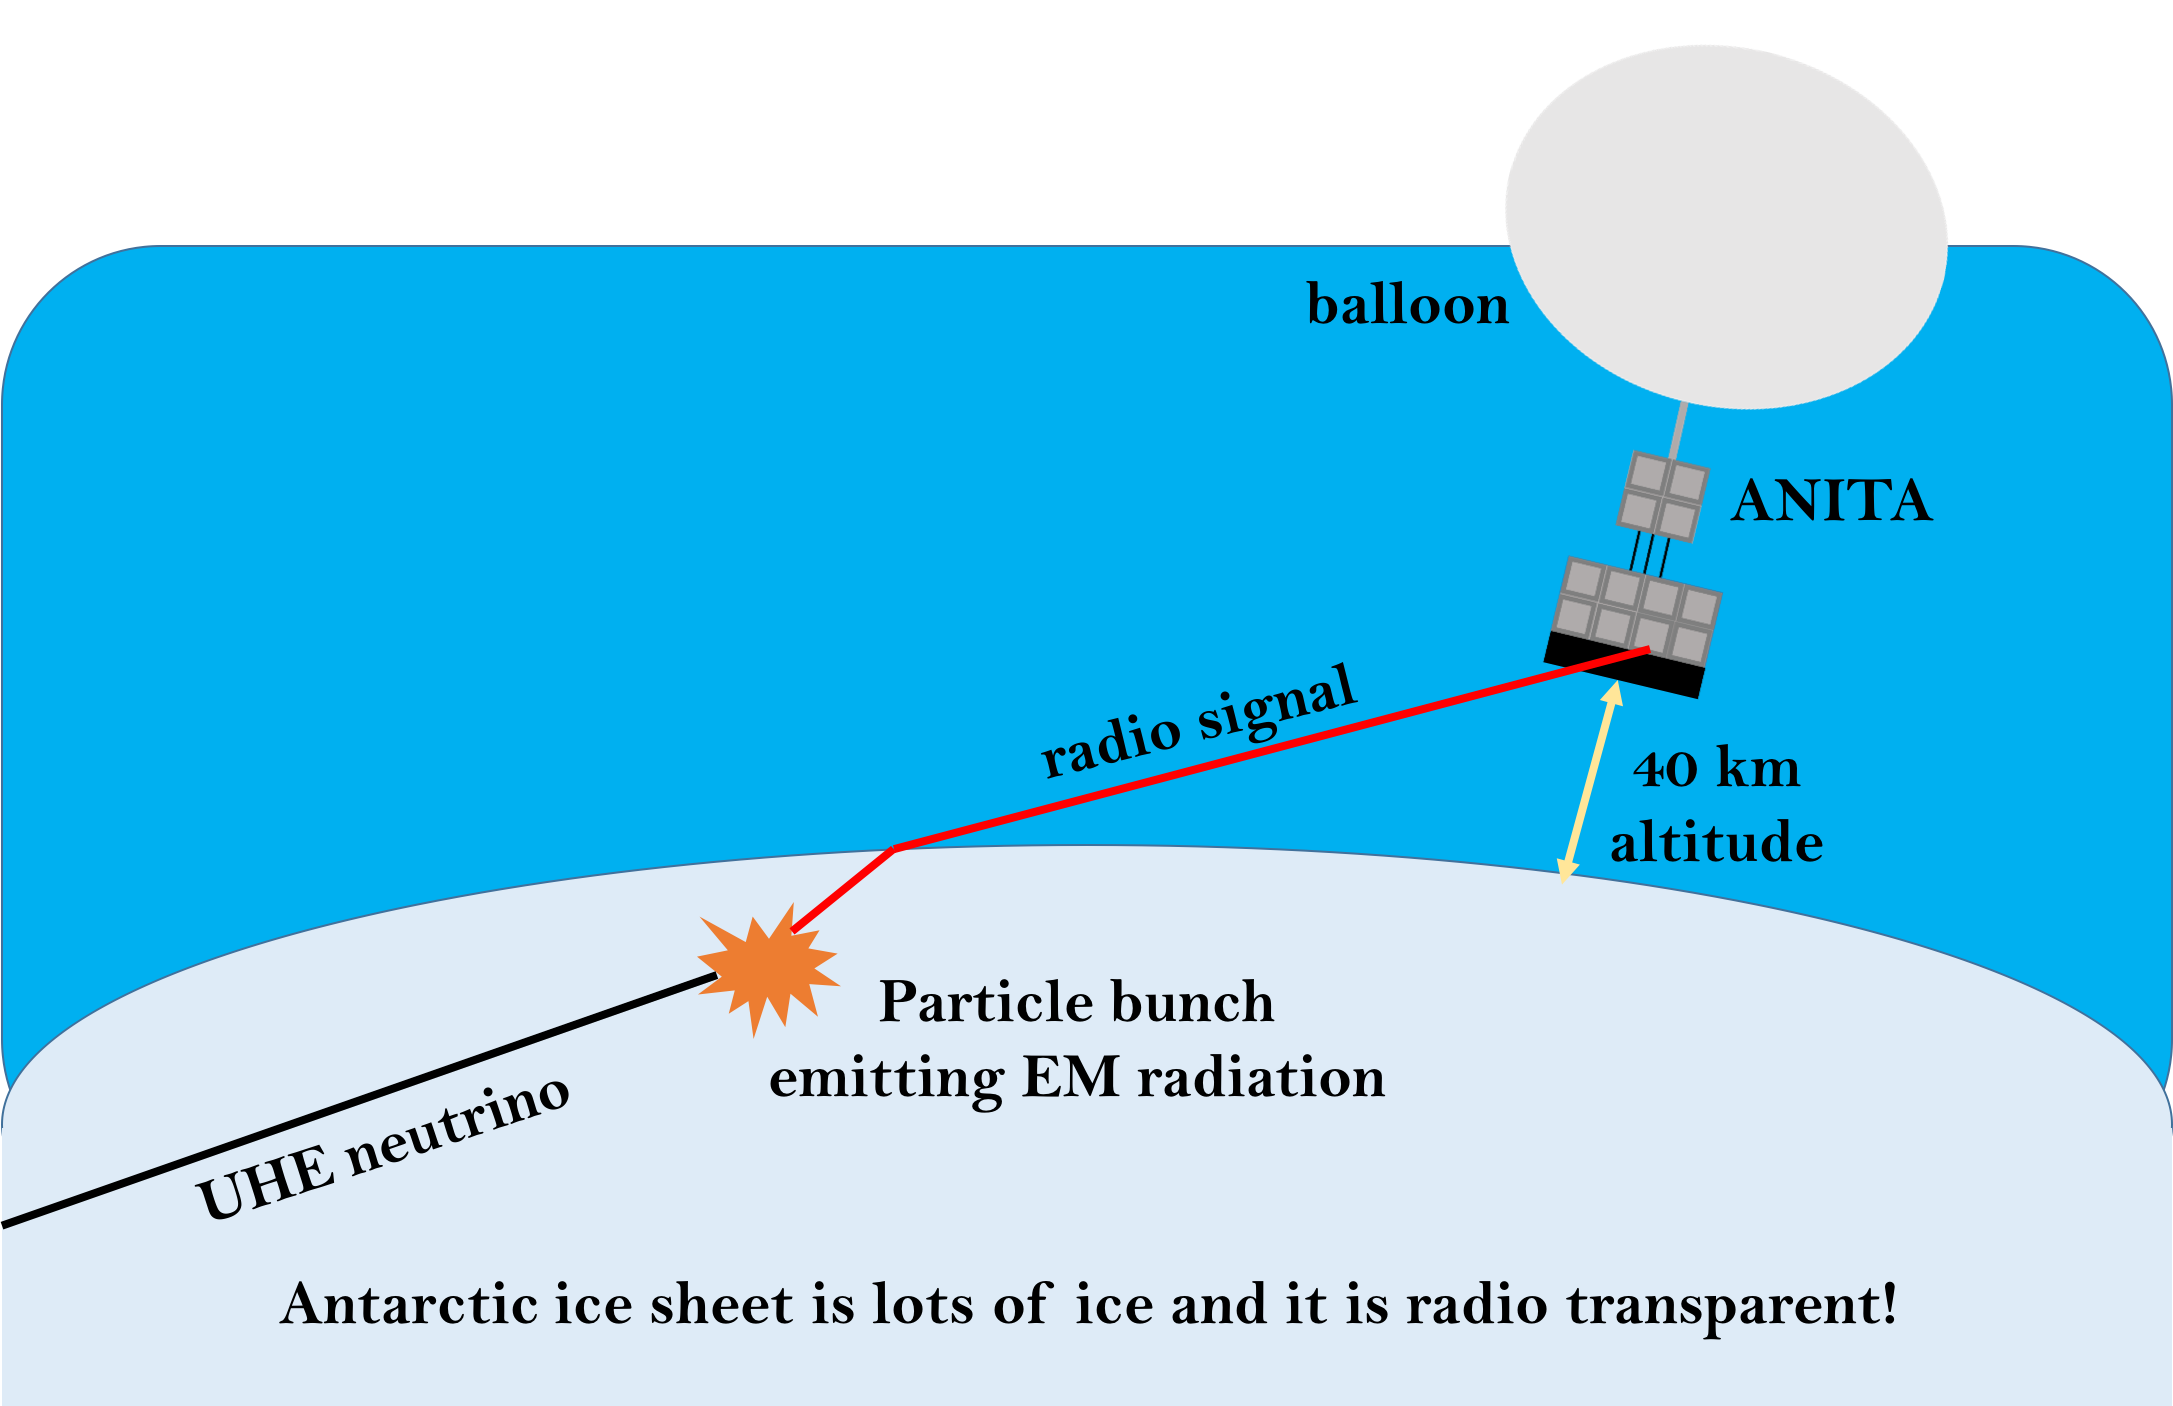
\includegraphics[width=0.9\textwidth]{figures/anita_cartoon_updated.png}
\caption{Concept of detection of UHE neutrinos with ANITA.}
\label{anita_cartoon}
\end{figure}


\chapter{Two-source high harmonic generation}
\label{two_source}

\section{Introduction}
\label{intro_ts}

A common difficulty in working with extreme ultraviolet (XUV) light is the lack of efficient and broadband optics, especially beam splitters. Here, we introduce a method for generating two sources of XUV light by high harmonic generation using a phase grating.  This phase grating allows for precise and stable control of the phase delay between the two generate XUV beams.  This can be thought of as an inline interferometer, and it can have applications for XUV Fourier transform spectroscopy, as well as transient absorption spectroscopy \cite{diffuse}.

\section{Theory}
\label{theory_ts}

In order to generate two ostensibly identical XUV pulses, we take advantage of a diffractive optical element known as a beam splitting grating.   The idea is to introduce a periodic phase step in the beam, which will cause the beam to diffract into different orders.  The phase step is designed such that the +1 and -1 orders are most efficiently populated, with an efficiency of up to 81$\%$.  These will be used to generate spatially separated harmonics.

A key advantage to this method is that it allows for control of the relative phase between the two sources generating harmonics.  By translating the grating relative to the beam, the relative phase difference between the +1 and -1 orders goes from -2$\pi$ to 2$\pi$.  This can be seen in the phase of the electric field at the focus:



\begin{figure}
	\centering
	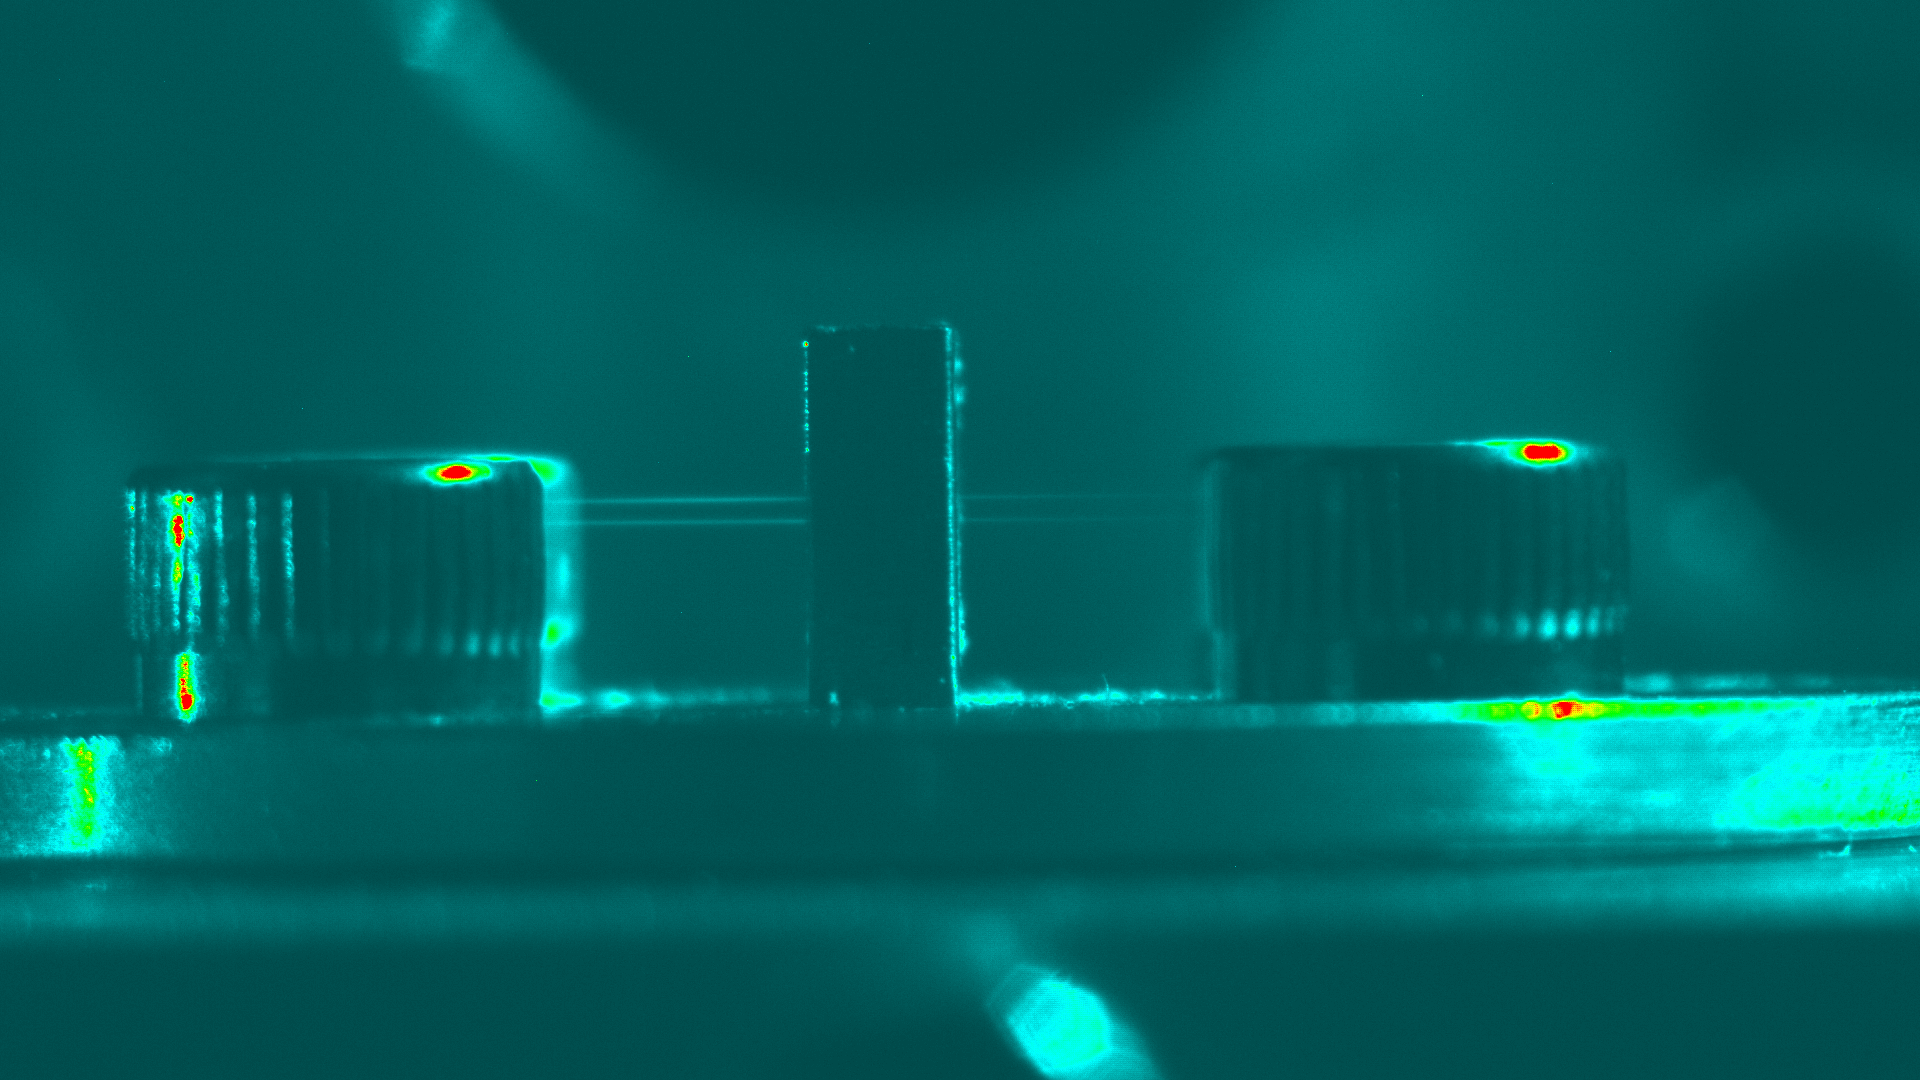
\includegraphics[width=0.9\textwidth]{figures/Two_source/ts_filament_gas_cell.png}
	\caption{Camera image of two sources generating a filament in a gas cell. Image was taken while chamber was vented and at ambient pressure.}
	\label{my_anita}
\end{figure}

\lipsum

\begin{figure}
	\centering
	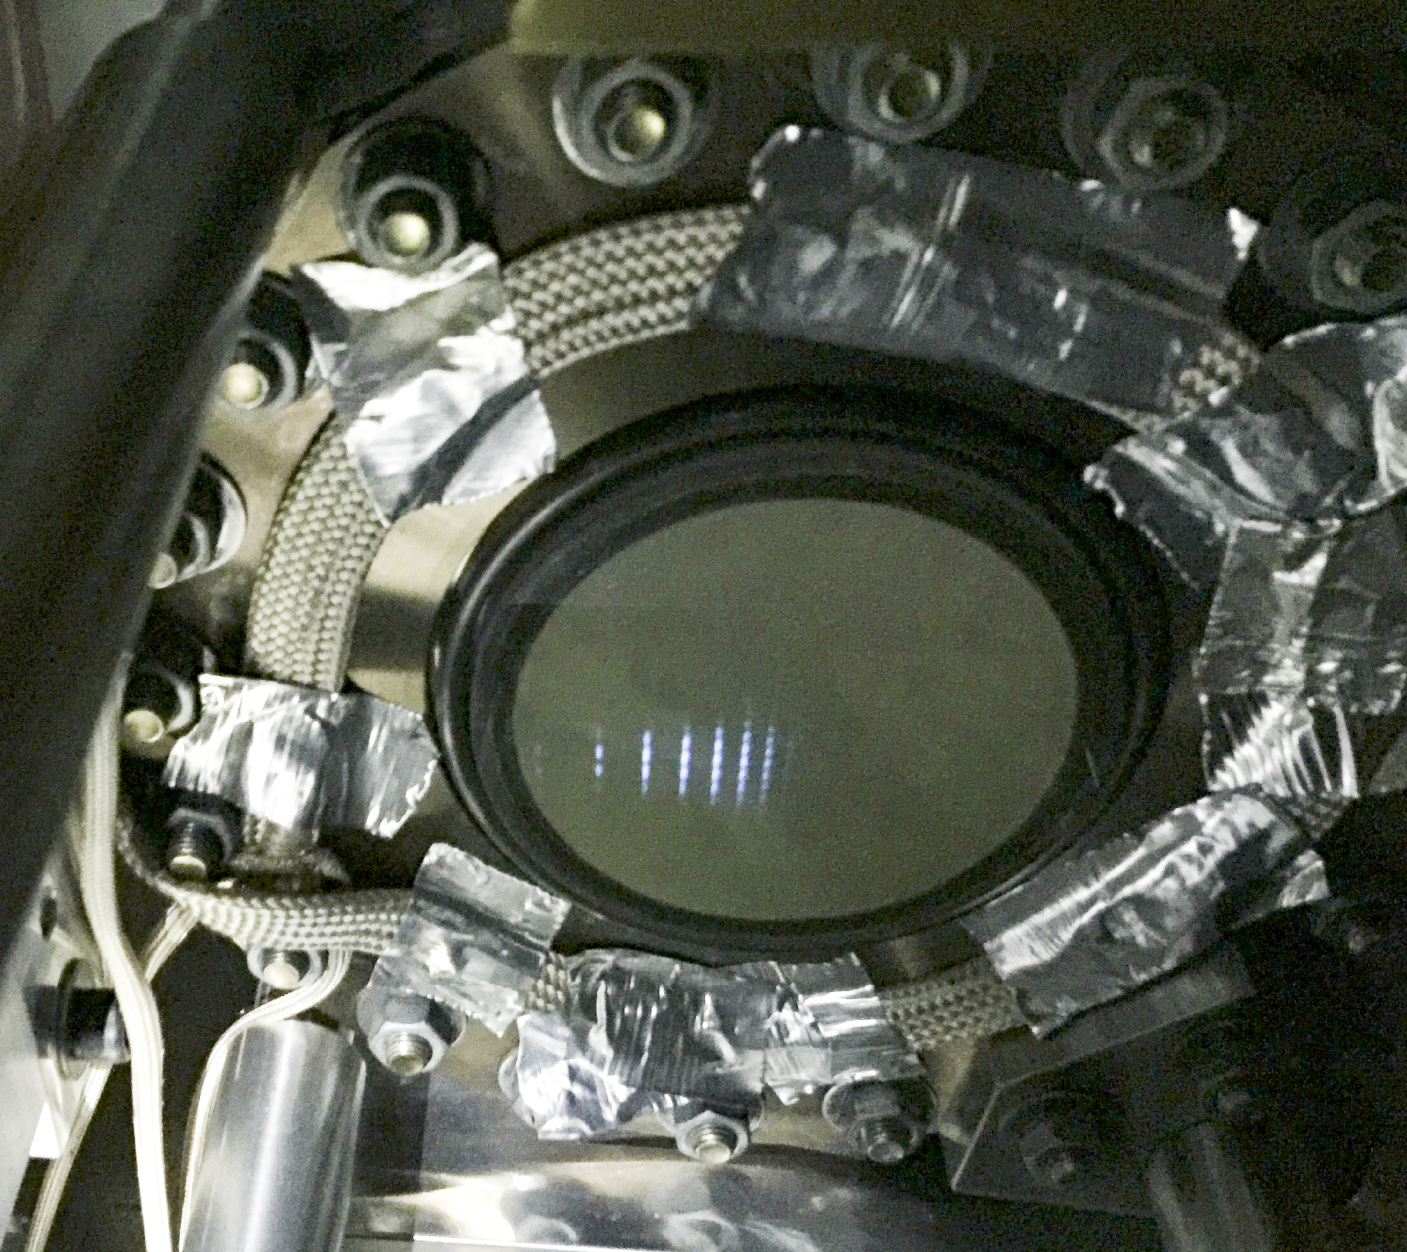
\includegraphics[width=0.9\textwidth]{figures/Two_source/MCP_ts_harmonics.png}
	\caption{Camera image of the output of the phosphor screen.  Harmonics are visible by eye.}
	\label{MCP_ts_harmonics}
\end{figure}

\lipsum

\begin{figure}
	\centering
	\includegraphics[width=0.9\textwidth]{figures/Two_source/dOD_dn.pdf}
	\caption{Camera image of two sources generating a filament in a gas cell. Image was taken while chamber was vented and at ambient pressure.}
	\label{my_anita}
\end{figure}

\lipsum
\begin{appendices}
\chapter{Square-wave Phase Grating}



           

\end{appendices}

\backmatter
% We use BIBTeX for the bibliography---you don't have to
%\nocite{*} % To display all refs, even uncited refs (useful when editting)
\bibliography{dissbib}
\bibliographystyle{unsrt} % use your favorite BIBTeX style

% If for some reason you are anti-BIBTeX, then you would use the
% following instead of the above:
%\begin{thebibliography}{99}
% ...
%\end{thebibliography}


% Note: GS 2010 requires bibliography/references _before_ the appendix
% if you believe their guidelines; however, conversations with GS
% staff suggests _they don't care_. Go figure. So do what you like.

%\appendix
%\include{app1}
%\include{app2}

\end{document}
